\chapter{Implementacija i korisničko sučelje}
		
		
		\section{Korištene tehnologije i alati}
			
			U nastavku su navedene tehnologije i alati koje smo koristili za izradu dokumentacije i aplikacije.
			\begin{itemize}
			\item\textbf{PgAdmin}\footnote{\url{https://www.pgadmin.org/}}je open-source alat za upravljanje bazama podataka PostgreSQL. Koristi se za sve osnovne operacije na bazi podataka, kao što su kreiranje, ažuriranje i brisanje tablica te postavljanje SQL upita. Ovaj alata omogućuje i napredne operacije, poput izvoza i uvoza podataka, upravljanja sigurnosnim ovlastima te optimizacije performansi.
			
			\item\textbf{React}\footnote{\url{https://reactjs.org/}}je JavaScript biblioteka za izradu web sučelja (frontend razvoj). Koristi se za izgradnju dinamičnih i interaktivnih web stranica i aplikacija koje reagiraju na korisničke interakcije. React je jednostavan za učenje i korištenje, a također je vrlo fleksibilan.
			
			\item\textbf{Spring Boot}\footnote{\url{https://spring.io/projects/spring-boot}} je open-source framework za Java backend razvoj. Koristi se za izgradnju RESTful web servisa i mikroservisa, kao i za automatizaciju mnogih zadataka koji su inače potrebni za izgradnju web servisa (kao što su konfiguracija, upravljanje ovisnostima i sigurnost). Spring Boot je iznimno popularan zbog svoje jednostavnosti i brzine.
			
			\item\textbf{GitHub}\footnote{\url{https://github.com/}} je web platforma za upravljanje izvornim kodom. Koristi se za spremanje, dijeljenje i suradnju na kodu.
			
			\item\textbf{WhatsApp}\footnote{\url{https://www.whatsapp.com/}} je popularna mobilna aplikacija za razmjenu poruka. Koristi se za komunikaciju unutar tima pomoću tekstualnih, glasovnih ili video poruka. WhatsApp je jednostavna moderna aplikacija koja na pouzdan način omogućava komunikaciju u realnom vremenu.
			
			\item\textbf{Visual Paradigm Online}\footnote{\url{https://online.visual-paradigm.com/}} je online alat za izradu UML dijagrama. Koristi se za modeliranje softverskih i drugih sustava. Ovaj je alat jednostavan za korištenje i ima široku paletu funkcionalnosti. 
			
			\item\textbf{Latex}\footnote{\url{https://www.latex-project.org/}} je programski jezik za pisanje strukturiranih tekstova i njihov automatski slog i prijelom u dokumente profesionalne kvalitete spremne za tisak. Omogućuje precizno kontroliranje izgleda dokumenta, uključujući veličinu i oblik slova, razmake, margine i druge elemente. LaTeX je popularan među znanstvenicima i inženjerima za pisanje tehničkih dokumenata.
			\end{itemize}
			
			\textbf{Zaključak}\\
			U izradi dokumentacije i aplikacije korištene su suvremene tehnologije i alati koji su omogućili izgradnju kvalitetnog i funkcionalnog proizvoda.
			
			
		
	
		\section{Ispitivanje programskog rješenja}
			
			\textbf{\textit{dio 2. revizije}}\\
	
			
			\subsection{Ispitivanje komponenti}
			\textit{Potrebno je provesti ispitivanje jedinica (engl. unit testing) nad razredima koji implementiraju temeljne funkcionalnosti. Razraditi \textbf{minimalno 6 ispitnih slučajeva} u kojima će se ispitati redovni slučajevi, rubni uvjeti te izazivanje pogreške (engl. exception throwing). Poželjno je stvoriti i ispitni slučaj koji koristi funkcionalnosti koje nisu implementirane. Potrebno je priložiti izvorni kôd svih ispitnih slučajeva te prikaz rezultata izvođenja ispita u razvojnom okruženju (prolaz/pad ispita). }
			
			
			
			\subsection{Ispitivanje sustava}
			
						\textbf{Test 1: Osnovne funkcije razreda User.}\\
			U ovom testu provjeravamo hoće li naš razred u konstruktoru dobro "zapamtiti" vrijednosti parametara, koje kasnije dohvaćamo get metodama. Primjer korištenja je pri registraciji.
			\begin{lstlisting}
				@Test
				void getterTest(){
					User user = new User("korisnik1", "ime", "prezime", "lozinka", "ime.prezime@gmail.com", null, "COMPETITOR");
					assertEquals("korisnik1", user.getUsername());
					assertEquals("ime", user.getName());
					assertEquals("prezime", user.getLastname());
					assertEquals("lozinka", user.getPassword());
					assertEquals("ime.prezime@gmail.com", user.getEmail());
					assertEquals(null, user.getImage());
					assertEquals(UserType.COMPETITOR, user.getUserType());	
				}
			\end{lstlisting}
			
			\textbf{Test 2: Osnove funkcije razreda Problem i Competition}\\
			U ovom primjeru provjeravamo možemo li stvoriti novi problem (zadatak), novi competition (natjecanje) te možemo li dodati problem u competition. Primjer korištenja je pri stvaranju natjecanja, odabiremo koji zadatci će biti dio tog natjecanja.
			\begin{lstlisting}
				@Test
				void competitionGetProblemsTest(){
					Map<String,String> mapa = new HashMap<>();
					mapa.put("ulaz", "izlaz");
					
					Problem problem = new Problem("1", "naslov", 5, "10:00", "text" , mapa, false, ProblemType.HARD);
					User user = new User("korisnik1", "ime", "prezime", "lozinka", "ime.prezime@gmail.com", null, "COMPETITION_LEADER");
					Set<Problem> set = new HashSet<>();
					set.add(problem);
					Competition competition = new Competition(user, LocalDateTime.now(), LocalDateTime.now(), set, null, false, false);
					assertEquals(set, competition.getProblems());
				}
			\end{lstlisting}
			
			\textbf{Test 3: Provjera sličice pehara.}\\
			U ovom primjeru provjeravamo slučaj kada neko natjecanje nema sličicu trofeja. Primjer korištenja je pri prikaza statistike natjecatelja. U slučaju da nema sličice pehara, prikazuje se "default" ikona pehara.
			\begin{lstlisting}
				@Test
				void competitionNoTrophyPictureThrowsTest(){
					Map<String,String> mapa = new HashMap<>();
					mapa.put("ulaz", "izlaz");
					
					Problem problem = new Problem("1", "naslov", 5, "10:00", "text" , mapa, false, ProblemType.HARD);
					User user = new User("korisnik1", "ime", "prezime", "lozinka", "ime.prezime@gmail.com", null, "COMPETITION_LEADER");
					Set<Problem> set = new HashSet<>();
					set.add(problem);
					Competition competition = new Competition(user, LocalDateTime.now(), LocalDateTime.now(), set, null, false, false);
					assertThrows(NullPointerException.class, () ->  competition.getTrophyPicture().getData());
				}
			\end{lstlisting}
			
			\textbf{Test 4: Provjera kompleksnijih funkcija sustava.}\\
			U ovom primjeru provjeravamo može li baza podataka dohvatiti nekog korisnika. Provjeru radimo uspoređivanjem savedUser.id (nalazi se u bazi podataka) i jsonNode.get("id"). JsonNode je objekt koji predstavlja odgovor na naš get zahtjev na server, ta metoda bi trebala iz baze podataka dohvatiti korisnika s id-em. Nakon dohvata korisnika provjeravamo je li get metoda vratila točan podatak. 
			\begin{lstlisting}
				@Test
				@DirtiesContext
				void testGetUserById() throws Exception{
					User user = new User("korisnik1", "ime", "prezime", "lozinka", "ime.prezime@gmail.com", null, "COMPETITION_LEADER");
					userRepository.delete(user);
					User savedUser = userRepository.save(user);
					MvcResult result = mockMvc.perform(get("/users/byId/{id}", savedUser.getId()))
					.andExpect(status().isOk())
					.andReturn();
					userRepository.deleteById(savedUser.getId());
					
					ObjectMapper objectMapper = new ObjectMapper();
					JsonNode jsonNode = objectMapper.readTree(result.getResponse().getContentAsString());
					
					assertEquals(savedUser.getId(), jsonNode.get("id").asLong());
				}
			\end{lstlisting}
			
			\textbf{Test 5: Provjera put metode pri stvaranju korisnika.}\\
			U ovom primjeru provjeravamo, slično kao u prošlom primjeru, hoće li get metoda vratiti dobrog korisnika. Korisnika ne upisujemo direktno u bazu v
			\begin{lstlisting}
				@Test
				@DirtiesContext
				void createUserTest() throws Exception{
					MockMultipartFile file = new MockMultipartFile(
					"image",           // Parametar "image" iz metode
					"filename.jpg",    // Naziv datoteke
					MediaType.IMAGE_JPEG_VALUE, // Tip datoteke
					"file content".getBytes()   
					);
					
					MvcResult resultFromCreateUser = mockMvc.perform(MockMvcRequestBuilders.multipart("/users")
					.file(file)
					.param("name", "ime2")
					.param("lastname", "prezime2")
					.param("username", "korisnik2")
					.param("email", "ime.prezime2@gmail.com")
					.param("password", "lozinka2")
					.param("userType", "COMPETITION_LEADER"))
					
					.andExpect(status().isOk())
					.andReturn();
					
					User userFromDatabase = userRepository.findByUsername("korisnik2");
					
					MvcResult resultFromGetUser = mockMvc.perform(get("/users/byId/{id}", userFromDatabase.getId()))
					.andExpect(status().isOk())
					.andReturn();
					
					
					ObjectMapper objectMapper = new ObjectMapper();
					JsonNode jsonNode = objectMapper.readTree(resultFromGetUser.getResponse().getContentAsString());
					userRepository.delete(userFromDatabase);
					assertEquals(userFromDatabase.getId(), jsonNode.get("id").asLong());
				}
			\end{lstlisting}
			
			\textbf{Test 6: Provjera uvjete za stvaranje korisnika.}\\
			U ovom primjeru pokušavamo stvoriti dva korisnika s istim korisničkim imenom (što narušava integritet baze podataka) te provjeravamo hoće li nam server to dopustiti ili vratiti pogrešku. Primjer korištenja je pri prijavi korisnika.
			\begin{lstlisting}
				@Test
				void uniqueUsernameTest() throws  Exception{
					MockMultipartFile file = new MockMultipartFile(
					"image",           // Parametar "image" iz metode
					"filename.jpg",    // Naziv datoteke
					MediaType.IMAGE_JPEG_VALUE, // Tip datoteke
					"file content".getBytes()   
					);
					
					MvcResult resultFromCreateUser = mockMvc.perform(MockMvcRequestBuilders.multipart("/users")
					.file(file)
					.param("name", "ime3")
					.param("lastname", "prezime3")
					.param("username", "korisnik3")
					.param("email", "ime.prezime3@gmail.com")
					.param("password", "lozinka3")
					.param("userType", "COMPETITION_LEADER"))
					
					.andExpect(status().isOk())
					.andReturn();
					MvcResult resultFromCreateUser2 = mockMvc.perform(MockMvcRequestBuilders.multipart("/users")
					.file(file)
					.param("name", "ime3")
					.param("lastname", "prezime3")
					.param("username", "korisnik3")
					.param("email", "ime.prezime4@gmail.com")
					.param("password", "lozinka3")
					.param("userType", "COMPETITION_LEADER"))
					.andReturn();
					ObjectMapper objectMapper = new ObjectMapper();
					User userKojegBrisem = userRepository.findByUsername("korisnik3");
					userRepository.deleteById(userKojegBrisem.getId());
					assertTrue(resultFromCreateUser2.getResponse().getStatus() == 400);
					
				}	
			\end{lstlisting}
			
			Primjer svih uspješno izvršenih testova:
			\begin{figure}[H]
				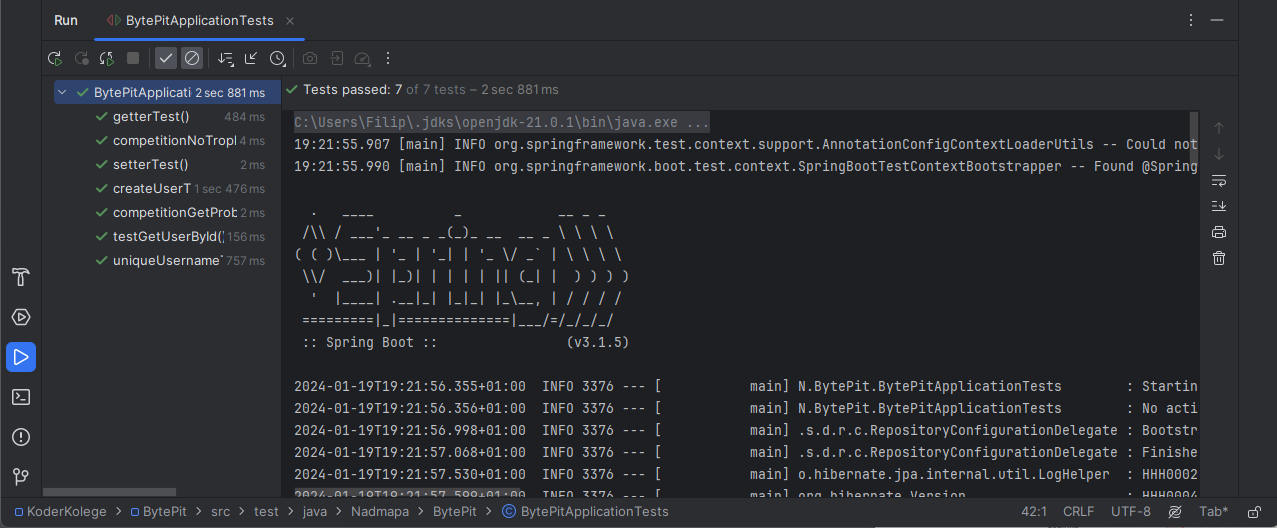
\includegraphics[scale=0.6]{slike/test1}
				%veličina slike u odnosu na originalnu datoteku i pozicija slike
				\centering
				\caption{Uspješno izvedeni testovi}
				\label{fig:uspjeh}
			\end{figure}
			
			Uzmimo za primjer Test 1, u slučaju da želimo simulirati pogrešno izršen test, umjesto koriskičkog imena "korisnik1" postat ćemo "korisnik"
			Primjer neuspješno izvršenog testa:
			\begin{figure}[H]
				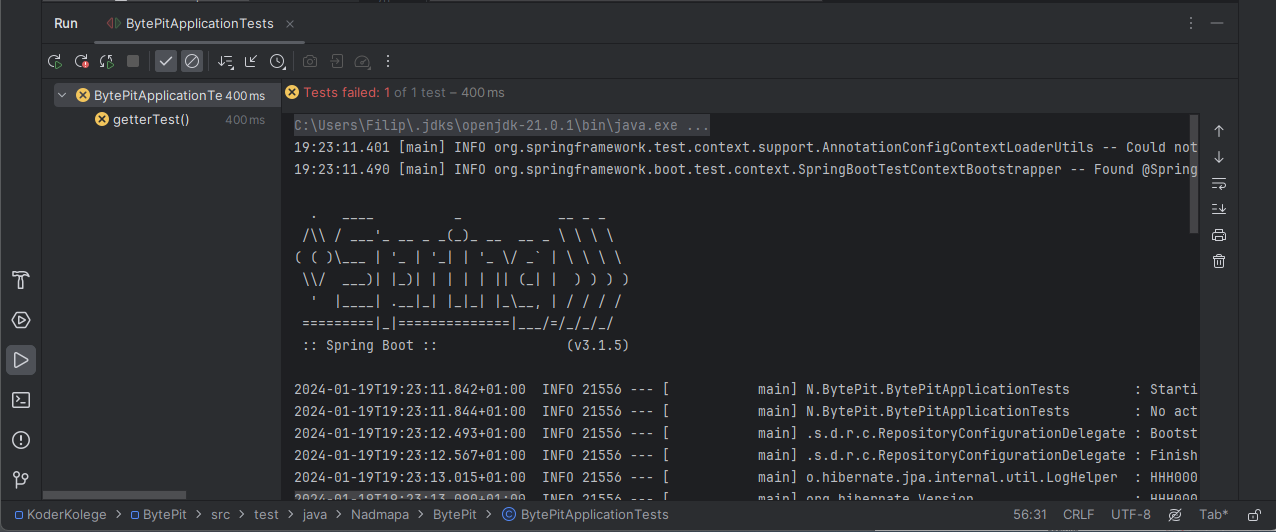
\includegraphics[scale=0.6]{slike/test2}
				%veličina slike u odnosu na originalnu datoteku i pozicija slike
				\centering
				\caption{Ne uspješno izvedeni testovi}
				\label{fig:neuspjeh}
			\end{figure}
			
			\begin{lstlisting}
				@Test
				void getterTest(){
					User user = new User("korisnik1", "ime", "prezime", "lozinka", "ime.prezime@gmail.com", null, "COMPETITOR");
					assertEquals("korisnik", user.getUsername());
					assertEquals("ime", user.getName());
					assertEquals("prezime", user.getLastname());
					assertEquals("lozinka", user.getPassword());
					assertEquals("ime.prezime@gmail.com", user.getEmail());
					assertEquals(null, user.getImage());
					assertEquals(UserType.COMPETITOR, user.getUserType());	
				}
			\end{lstlisting}
			
			
			 
			 \textit{Izradu ispitnih slučajeva pomoću radnog okvira Selenium moguće je provesti pomoću jednog od sljedeća dva alata:}
			 \begin{itemize}
			 	\item \textit{dodatak za preglednik \textbf{Selenium IDE} - snimanje korisnikovih akcija radi automatskog ponavljanja ispita	}
			 	\item \textit{\textbf{Selenium WebDriver} - podrška za pisanje ispita u jezicima Java, C\#, PHP koristeći posebno programsko sučelje.}
			 \end{itemize}
		 	\textit{Detalji o korištenju alata Selenium bit će prikazani na posebnom predavanju tijekom semestra.}
			
			\eject 
		
		
		\section{Dijagram razmještaja}
		
		\noindent{
			UML-dijagrami razmještaja su vrsta strukturnih UML- dijagrama koji prikazuju fizicku arhitekturu i konfiguraciju razmještaja programskog sustava.
			
			U ovoj aplikaciji korisnikovo računalo preko web preglednika pristupa poslužiteljovom računalu pomoču HTTP protokola. Na poslužiteljskom računalu se nalazi naša aplikacija BytePit i baza podataka s kojom aplikacija komunicira. Sustav je baziran na arhitekturi ”klijent – posluzitelj”
		}\\
			
			\begin{figure}[H]
				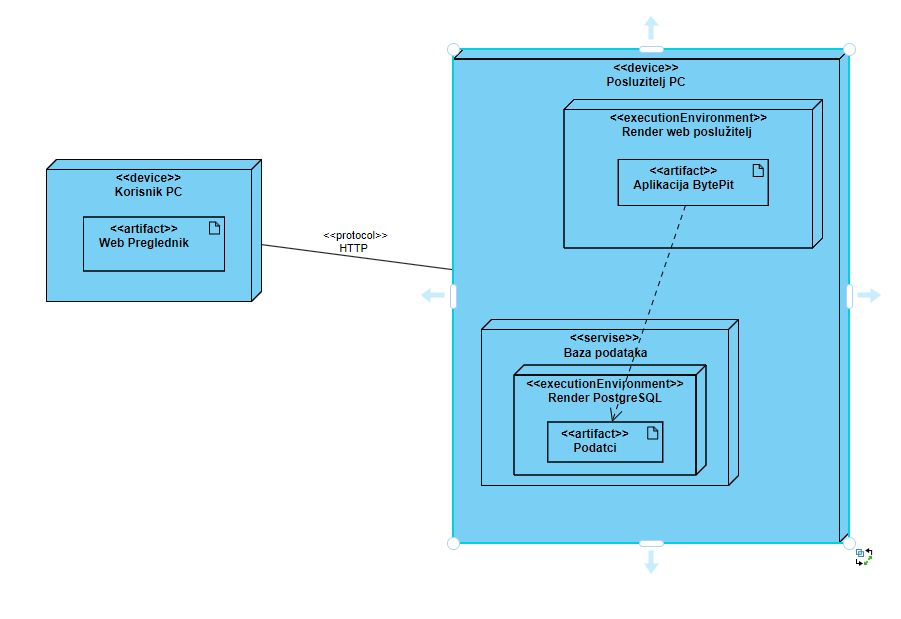
\includegraphics[scale=0.6]{slike/Dijagram razmjestaja}
				%veličina slike u odnosu na originalnu datoteku i pozicija slike
				\centering
				\caption{Dijagram razmjestaja}
				\label{fig:dijagramrazmjestaja}
			\end{figure}
		
		\section{Upute za puštanje u pogon}
 
			
			Postavljanje aplikacije u pogon putem usluge Render zahtijeva pažljivo provedene korake uključujući kreiranje baze podataka, kreiranje backend-a  te kreiranje frontenda, čime se osigurava siguran i učinkovit deploy.
			
			Prije samog puštanja aplikacije u pogon potrebno je provesti tri ključna koraka:
			\begin{packed_enum}
				\item \textbf{Konfiguracija baze podataka}
				\begin{itemize}
					\item Ovaj proces uključuje definiranje environmental varijabli unutar konfiguracije razvojnog okruženja (IDE). U našem slučaju, konfiguracija se nalazi u datoteci src/main/resources/application.properties. U ovoj datoteci specificiramo parametre kao što su korisničko ime, lozinka, URL baze podataka te određujemo port poslužitelja. Primjer konfiguracije:
					\begin{figure}[H]
						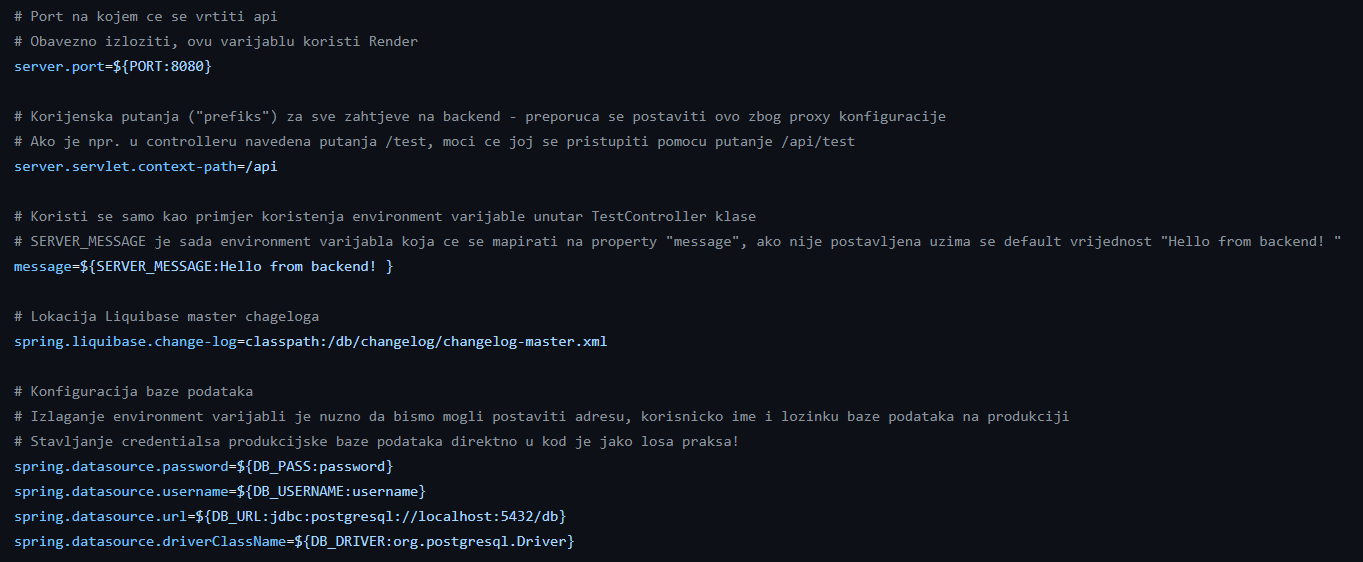
\includegraphics[scale=0.5]{slike/EnvironmentVarijable}
						%veličina slike u odnosu na originalnu datoteku i pozicija slike
						\centering
						\caption{Environment Varijable u IDE-u}
						\label{fig:EnvVar}
					\end{figure}
					
						
				\end{itemize}
				\item \textbf{Priprema backend-a za deploy}
				\begin{itemize}
					\item Nakon postavljanja baze podataka, slijedi priprema backend-a za deploy. Ovaj korak uključuje dodavanje Dockerfile skripte za izgradnju i pokretanje aplikacije.  U našem slučaju, koristimo Maven, pa je Dockerfile konfiguriran na sljedeći način:
					\begin{lstlisting}
						# Container za izgradnju (build) aplikacije
						FROM openjdk:17-alpine AS builder
						
						# Kopiranje izvornog koda u container
						COPY ../../.mvn .mvn
						COPY ../../mvnw .
						COPY ../../pom.xml .
						COPY ../../src src
						RUN chmod +x mvnw
						
						# Pokretanje builda
						RUN ./mvnw clean package
						
					
						FROM openjdk:17-alpine
						
						COPY --from=builder target/*.jar /app.jar
						
						EXPOSE 8080
						
						ENTRYPOINT ["java","-jar","/app.jar"]
						
					\end{lstlisting}
					\item Ukoliko se mijenja lokacija Dockerfilea paziti na putanje unutar COPY naredbi u Dockerfile skripti. U nasem slucaju Docker file se nalazi u root direktoriju Docker/Maven/Dockerfile te su po toj putanji pisane naredbe COPY.
				\end{itemize}
				
				\item \textbf{Priprema frontenda za deploy}
				\begin{itemize}
					\item Potrebno je dodati potrebne dependencije u package.json datoteku. U terminalu je potrebno izvršiti sljedeće naredbe:
					\begin{lstlisting}
						npm install http-proxy-middleware
						npm install dotenv
						npm install express
					\end{lstlisting}
					\item Potrebno je kreirati Proxy.js, u src direktorij, koji služi kao proxy server za lokalni development (preusmjeruje api pozive na localhost:8080). Ovo je primjer koda:
					\begin{lstlisting}
						const { createProxyMiddleware } = require("http-proxy-middleware");
						
						module.exports = function (app) {
							app.use(
							"/api",
							createProxyMiddleware({
								target: "http://localhost:8080/",
								changeOrigin: true,
							})
							);
						};
					\end{lstlisting}
					\item Stvoriti app.js, u root direktorij, koja sadrži Express server za produkcijski proxy i posluživanje frontenda. Ovo je primjer koda:
					\begin{lstlisting}
						const express = require("express");
						const { createProxyMiddleware } = require("http-proxy-middleware");
						require("dotenv").config();
						const path = require("path");
						
						const app = express();
						
						// Configuration
						const { PORT, HOST, API_BASE_URL } = process.env;
						
						// Proxy
						app.use(
						"/api",
						createProxyMiddleware({
							target: API_BASE_URL,
							changeOrigin: true,
						})
						);
						
						app.use(express.static(path.join(__dirname, 'build')));
						
						app.listen(PORT, HOST, () => {
							console.log(`Starting Proxy at ${HOST}:${PORT}`);
						});
						
						app.get("*", async (req, res) => {
							res.sendFile(path.join(__dirname, 'build', 'index.html'))
						});
						
					\end{lstlisting}
					\item Izmjeniti package.json skripte i dodati specifične konfiguracije:
					\begin{lstlisting}
						"build": "yarn install && react-scripts build",
						"start-prod": "node app.js",
						"engines": {
							"node": ">=18.18.0 <19.0.0"
						}
						
					\end{lstlisting}
				\end{itemize}
			\end{packed_enum}
			
			Sada, nakon završene pripreme, možemo započeti deploy.
			
				\begin{packed_enum}
				\item \textbf{Kreiranje baze podataka}
				U rander dashboardu:
				\begin{itemize}
					\item New \textrightarrow PostgreSQL
					\item Postaviti ime baze i opcionalno username za korisnika baze (password je automatski generiran)
					\item Region Frankfurt
					\item Create Database
				\end{itemize}
				
				\item \textbf{Kreiranje backend-a}
				U Render dashboardu:
				\begin{itemize}
					\item New \textrightarrow Web Service
					\item Povezati GitHub račun, nakon čega su za odabir dostupni svi projekti na koje imate prava pristupa
					\item Stisnuti connect pored odgovarajućeg projekta
					\item Postaviti ime za servis (postat ce dio web adrese)
					\item Postaviti root directory (u nasem slucaju: dev)
					\item Environment Docker
					\item Region Frankfurt
					\item Na dnu proširiti \textit{advanced}
					\item Dodati potrebne environment varijable (vidi sliku \ref{fig:EnvVar}), kopirati vrijednosti iz postavki baze na renderu (vidi sliku \ref{fig:postavkebaze}). Također dodati kopirane environment varijable u IDE okruzenje (vidi sliku \ref{fig:EnvVar})
					
					\begin{figure}[H]
						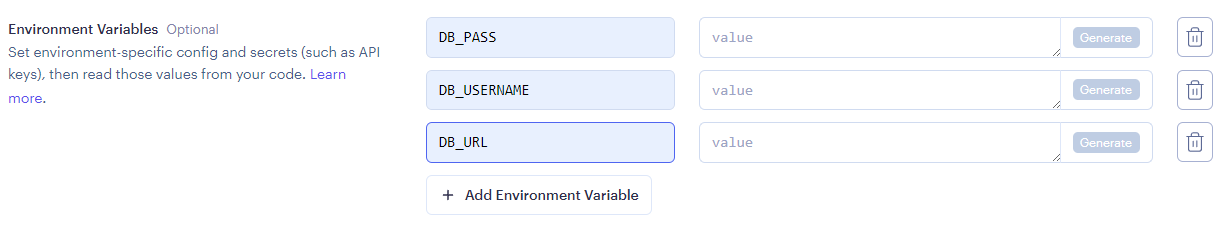
\includegraphics[scale=0.5]{slike/EnvironmentVarijableBackend}
						%veličina slike u odnosu na originalnu datoteku i pozicija slike
						\centering
						\caption{Environment Varijable za backend}
						\label{fig:EnvVarbackend}
					\end{figure}
					
					\begin{figure}[H]
						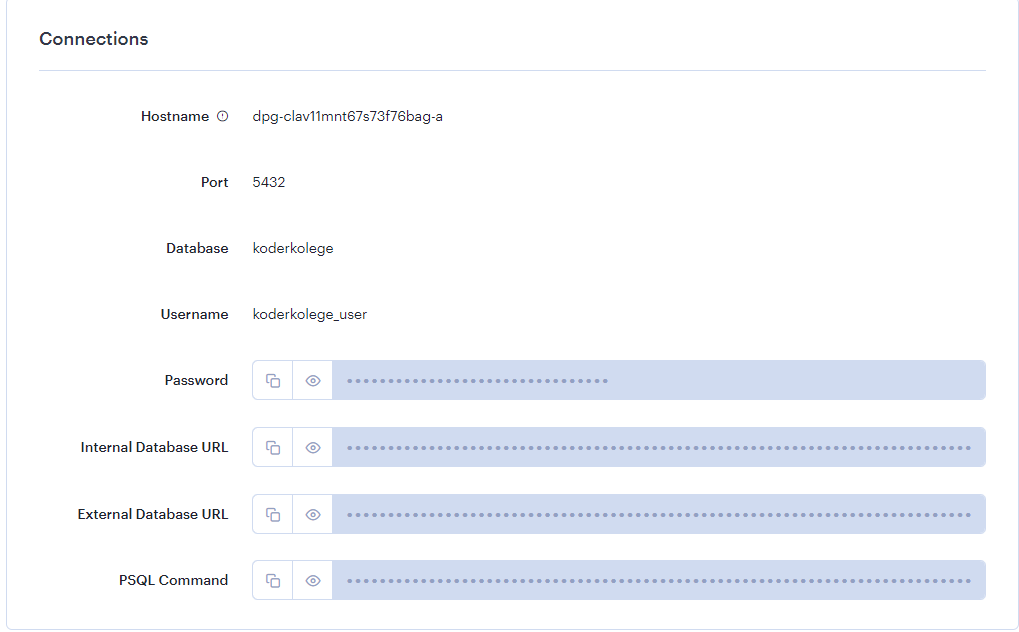
\includegraphics[scale=0.5]{slike/PostavkeBazePodataka}
						%veličina slike u odnosu na originalnu datoteku i pozicija slike
						\centering
						\caption{Postavke baze podataka na renderu}
						\label{fig:postavkebaze}
					\end{figure}
					\item Postaviti putanju za Dockerfile ovisno koji se package manager koristi (u ovom slučaju ./docker/maven/Dockerfile, vidi sliku \ref{fig:dockerfile})
					\begin{figure}[H]
						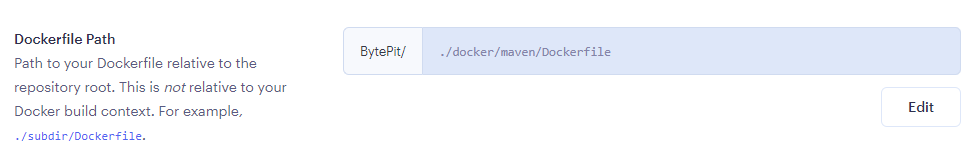
\includegraphics[scale=0.5]{slike/DockerFile}
						%veličina slike u odnosu na originalnu datoteku i pozicija slike
						\centering
						\caption{Putanja za Dockerfile}
						\label{fig:dockerfile}
					\end{figure}
					\item Stisnuti Create Web Service
				\end{itemize}
				
				\item \textbf{Kreiranje frontenda}
				\begin{itemize}
					\item New \textrightarrow Web Service
					\item Povezati GitLab racun, nakon cega su za odabir dostupni svi projekti na koje imate prava pristupa
					\item Stisnuti connect pored odgovarajućeg projekta
					\item Postaviti ime za servis (postat ce dio web adrese)
					\item Postaviti root directory (u nasem slucaju: dev)
					\item Environment Node
					\item Region Frankfurt
					\item Build Command postaviti na yarn build, a Start Command yarn start-prod (vidi sliku \ref{fig:BuildComand})
					\begin{figure}[H]
						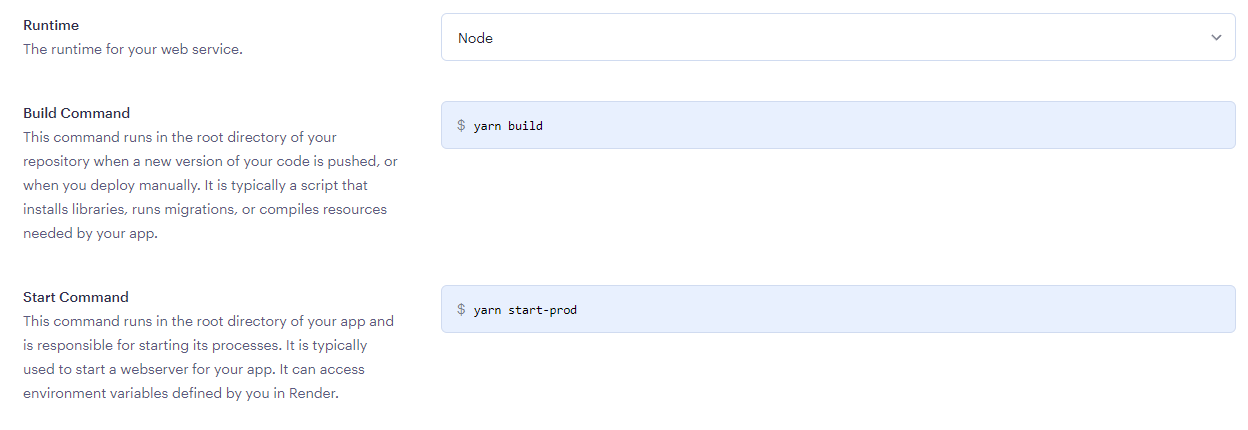
\includegraphics[scale=0.5]{slike/BuildComand}
						%veličina slike u odnosu na originalnu datoteku i pozicija slike
						\centering
						\caption{Build Comand za Node enviroment}
						\label{fig:BuildComand}
					\end{figure}	
					\item Na dnu proširiti \textit{advanced}
					\item Dodati potrebne environment varijable - API BASE URL postaviti na adresu deployanog backenda aplikacije dostupnu na Render dashboardu (vidi sliku \ref{fig:BuildComand})
						\begin{figure}[H]
							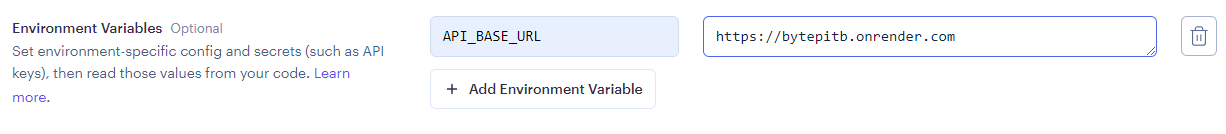
\includegraphics[scale=0.5]{slike/EnvironmentVarijableFront}
							%veličina slike u odnosu na originalnu datoteku i pozicija slike
							\centering
							\caption{Environment Varijable za frontend }
							\label{fig:EnvVarfront}
						\end{figure}
					\item Stisnuti Create Web Service
				\end{itemize}
			\end{packed_enum}
			
			Nakon uspješnog deploya, naša aplikacija sada bezbrižno operira na Render poslužitelju.
		
			
			
			